\documentclass{beamer}
\usepackage{tikz}
\usetikzlibrary{graphs, arrows, positioning}
\usepackage{graphicx}
\usepackage{amsmath}
\usepackage{pgfplots}
\usepackage{xcolor} % For colored elements
\usepackage{tcolorbox} % For boxed algorithm format

\usetheme{Madrid} % Applying a beamer theme with red header/footer
\usecolortheme{beaver} % Red color scheme
\definecolor{customred}{HTML}{A30000}
\setbeamercolor{title}{fg=white, bg=customred}

\title{Algorithm, Design \& Analysis}
\subtitle{\textcolor{white!70}{Lecture 18: Dijkstra’s Algorithm}}
\author{{ Muhammad Bilal    \&    Muhammad Asharib }}
\institute{Information Technology University}
\date{March 27, 2025}
\logo{\includegraphics[height=1cm]{university_logo}}
\begin{document}

\begin{frame}
    \titlepage
\end{frame}

\begin{frame}{About Your Fellows}
        \begin{itemize}
            \item Hi there! We are \textcolor{red}{\textbf{Asharib}} {and }\textcolor{red}{\textbf {Bilal}}.
            \item We are Associate Students at ITU.
        \end{itemize}
\end{frame}

\begin{frame}{Introduction to Dijkstra’s Algorithm}
    \begin{itemize}
        \item Used to find the shortest path from a single source to all vertices or a specified vertex in a weighted graph.
        \item Using a priority queue (min-heap) for efficient vertex selection.
        \item {\textcolor{blue}{Decrease-Key} heap operation is used to maintain an optimized priority queue.}
    \end{itemize}
    

    % Adjust positioning if needed
    \vfill % pushes what's below to bottom
    \hfill % pushes box to right
    \begin{minipage}{7cm}
        \begin{tcolorbox}[
            colback=gray!10,
            colframe=black!60,
            boxrule=0.5pt,
            width=6.5cm,
            halign=left
        ]
            \small Dijkstra works like a miser traveling the world—always taking the cheapest step forward to minimize cost.
        \end{tcolorbox}
    \end{minipage}
    
\end{frame}

\begin{frame}
    \centering
         \begin{tcolorbox}[
        colback=white, colframe=gray!20, boxrule=2mm, arc=5mm,
        width=0.8\textwidth]
     \centering
    \Large\textbf{\textcolor{customred}{What is Decrease Key}}
    \end{tcolorbox}
\end{frame}



\begin{frame}{Heap Operation – Decrease-Key}
    \textbf{Definition:}
    \begin{itemize}
        \item The decrease-key operation is used when an edge relaxation lowers the shortest known distance of a vertex.
        \item Helps update distances and maintains the heap property by sifting up updated elements.
    \end{itemize}
\end{frame}

% Step 1: Initial Heap
\begin{frame}{Step 1: Initial Min-Heap}

    \centering
    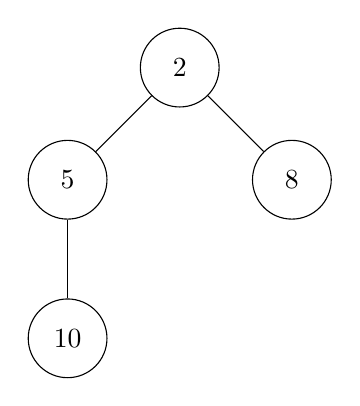
\begin{tikzpicture}[scale=1, every node/.style={circle,draw,minimum size=1cm}]
        \node (A) {2};
        \node (B) [below left=1cm of A] {5};
        \node (C) [below right=1cm of A] {8};
        \node (D) [below=1cm of B] {10};

        \draw (A) -- (B);
        \draw (A) -- (C);
        \draw (B) -- (D);
    \end{tikzpicture}
    \vspace{0.1cm}
\textbf{Before decrease-key:} The key at node 10 is reduced to 1.
\end{frame}

% Step 2: Key updated at the lowest level
\begin{frame}{Step 2: Update Key (10 → 1)}
    \centering
    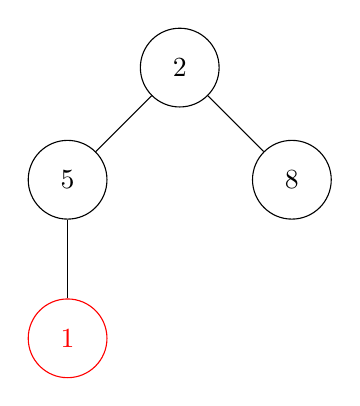
\begin{tikzpicture}[scale=1, every node/.style={circle,draw,minimum size=1cm}]
        \node (A) {2};
        \node (B) [below left=1cm of A] {5};
        \node (C) [below right=1cm of A] {8};
        \node (D) [below=1cm of B, color=red] {1}; % Highlight changed node

        \draw (A) -- (B);
        \draw (A) -- (C);
        \draw (B) -- (D);
    \end{tikzpicture}
    \vspace{0.5cm}
    \textbf{Key changed:} Node 10 is now 1. Heap property is violated.
\end{frame}

% Step 3: Sift-Up - Swapping with parent (5)
\begin{frame}{Step 3: Sift-Up (Swap 1 , 5)}
    \centering
    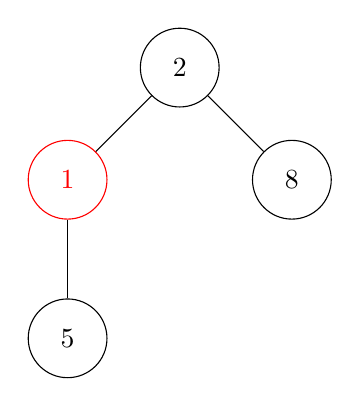
\begin{tikzpicture}[scale=1, every node/.style={circle,draw,minimum size=1cm}]
        \node (A) {2};
        \node (B) [below left=1cm of A, color=red] {1}; % Highlight swap
        \node (C) [below right=1cm of A] {8};
        \node (D) [below=1cm of B] {5};

        \draw (A) -- (B);
        \draw (A) -- (C);
        \draw (B) -- (D);
    \end{tikzpicture}
    \vspace{0.5cm}
    \textbf{Step:} Node 1 swaps with its parent (5).
\end{frame}

% Step 4: Sift-Up - Swapping with root (2)
\begin{frame}{Step 4: Sift-Up (Swap 1 , 2)}
    \centering
    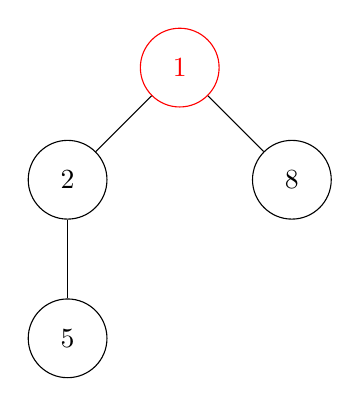
\begin{tikzpicture}[scale=1, every node/.style={circle,draw,minimum size=1cm}]
        \node (A) [color=red] {1}; % Highlight swap
        \node (B) [below left=1cm of A] {2};
        \node (C) [below right=1cm of A] {8};
        \node (D) [below=1cm of B] {5};

        \draw (A) -- (B);
        \draw (A) -- (C);
        \draw (B) -- (D);
    \end{tikzpicture}
    \vspace{0.5cm}
    \textbf{Step:} Node 1 swaps with its parent (2). Min-Heap property restored.
\end{frame}

\begin{frame}{Final Heap After Decrease-Key}
    \centering
    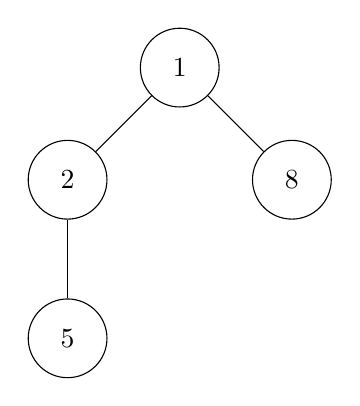
\begin{tikzpicture}[scale=1, every node/.style={circle,draw,minimum size=1cm}]
        \node (A) {1};
        \node (B) [below left=1cm of A] {2};
        \node (C) [below right=1cm of A] {8};
        \node (D) [below=1cm of B] {5};

        \draw (A) -- (B);
        \draw (A) -- (C);
        \draw (B) -- (D);
    \end{tikzpicture}
    \vspace{0.5cm}
    \textbf{Final Structure:} Min-Heap is now valid!
\end{frame}

\begin{frame}{Time Complexity Analysis}
    \begin{tcolorbox}[colback=gray!10,colframe=red!75!black,title=Time Complexity for Binary Heap]
    \begin{itemize}
        \item \textbf{Insert:} $O(\log N)$
        \item \textbf{Delete Min:} $O(\log N)$
        \item \textbf{Decrease Key:} $O(\log N)$
        
    \end{itemize}
    \end{tcolorbox}
\end{frame}

\begin{frame}
    \centering
     \begin{tcolorbox}[colback=white!10, colframe=gray!10, boxrule=2mm, arc=5mm, width=0.8\textwidth]
     \centering
    \Large\textbf{\textcolor{customred}{Back to Dijkstra's Algorithm}}
    \end{tcolorbox}
\end{frame}

\begin{frame}{Algorithm Explanation}
    \textbf{Initialization:}
    \begin{itemize}
        \item Set all distances except the source to infinity ($\infty$).
        \item Set the distance from the source to 0.
        \item Store all vertices in a min-heap based on their current shortest distances.
    \end{itemize}
    \textbf{Processing Nodes (Main Loop):}
    \begin{itemize}
        \item Extract the vertex $u$ with the smallest distance from the heap.
        \item Relax all its neighbors $v$:
        \begin{itemize}
            \item If a shorter path to $v$ is found through $u$, update $d[v]$.
            \item Update the predecessor of $v$ to track the shortest path.
            \item The decrease-key operation is used to update the heap efficiently.
        \end{itemize}
    \end{itemize}
\end{frame}

\begin{frame}{Pseudocode}
    \begin{tcolorbox}[colback=gray!10,colframe=red!75!black,title=Dijkstra’s Algorithm:]

    \begin{itemize}
            \item  $d[v] = \infty$ for all V.
            \item  $\pi[v] = \text{NIL}$ for all V.
            \item  $d[s] = \phi$
            \item H = Insert all vertices into a min-heap with their distances.
            \item For i = 1 to n:
            \begin{itemize}
                \item u = $deleteMin(H)$
                \item For all edges $(u, v)$:
                \begin{itemize}
                \item If $d[u] + w(u, v) < d[v]$:
                    \begin{itemize}
                    \item $d[v] = d[u] + w(u, v)$.
                    \item $\pi[v] = u$.
                    \item $decreaseKey(H,v,d[v])$
                    \end{itemize}
                \end{itemize}
            \end{itemize}
            
        
    \end{itemize}
    \end{tcolorbox}
\end{frame}

\begin{frame}{Dijkstra's Algorithm - Example}
    \begin{center}
        \begin{tikzpicture}[auto, node distance=2cm, thick, 
            main node/.style={circle, draw, fill=gray!10, font=\sffamily\bfseries, minimum size=1cm},
            label node/.style={fill=yellow, font=\sffamily\small, inner sep=2pt},
            >=stealth]

        % Define Nodes
        \node[main node] (S) {S};
        \node[main node] (A) [above right=of S] {A};
        \node[main node] (C) [right=of S] {C};
        \node[main node] (D) [below right=of S] {D};
        \node[main node] (E) [below right=of B, right=of D] {E};
        \node[main node] (B) [right=of C] {B};
        \node[main node] (F) [above right=of B] {F};
        \node[main node] (G) [right=of B] {G}; 

        % Define Edges with Weights
        \path[->, thick] (S) edge node[label node] {3} (A);
        \path[->, thick] (S) edge node[label node] {8} (C);
        \path[->, thick] (S) edge node[label node] {1} (D);
        \path[->, thick] (A) edge node[label node] {2} (C);
        \path[->, thick] (A) edge node[label node] {2} (F);
        \path[->, thick] (D) edge node[label node] {4} (C);
        \path[->, thick] (D) edge node[label node] {5} (E);
        \path[->, thick] (E) edge node[label node] {3} (B);
        \path[->, thick] (C) edge node[label node] {3} (B);
        \path[->, thick] (E) edge node[label node] {3} (G);
        \path[->, thick] (B) edge node[label node] {4} (G);
        \path[->, thick] (F) edge node[label node] {9} (B);
        \path[->, thick] (F) edge node[label node] {1} (G);

        \end{tikzpicture}
    \end{center}
\end{frame}


\begin{frame}{Example - Step by Step}
\node{
    \only<1>{\textbf{Step 1: Starting with S}}
    \only<2>{\textbf{Step 2: Updating Neighbors of S}}
    \only<3>{\textbf{Step 3: Selecting D(Smallest Distance)}}
    \only<4>{\textbf{Step 4: Updating Neighbors of D}}
    \only<5>{\textbf{Step 5: Selecting A(Smallest Distance)}}
    \only<6>{\textbf{Step 6: Updating Neighbors of A}}
    \only<7>{\textbf{Step 7: Selecting F(Smallest Distance)}}
    \only<8>{\textbf{Step 8: Updating Neighbors of F}}
    \only<9>{\textbf{Step 9: Selecting C(Smallest Distance)}}
    \only<10>{\textbf{Step 10: Updating Neighbors of C}}
    \only<11>{\textbf{Step 11: Selecting G :Smallest Distance(Goal Reached!)}}
};

\begin{tikzpicture}[auto, node distance=2cm, thick, 
    main node/.style={circle, draw, fill=gray!10, font=\sffamily\bfseries, minimum size=1cm},
    visited node/.style={circle, draw, fill=red!50,font=\sffamily\bfseries, minimum size=1cm},
    eliminated node/.style={circle, draw, fill=gray!30, font=\sffamily\bfseries, minimum size=1cm},
    label node/.style={fill=yellow, font=\sffamily\small, inner sep=2pt},
    edge highlight/.style={draw=red, very thick},
    update edge/.style={draw=green, dashed, thick},
    >=stealth]

% Define Nodes
\node[main node] (S) {S};
\node[main node] (A) [above right=of S] {A};
\node[main node] (C) [right=of S] {C};
\node[main node] (D) [below right=of S] {D};
\node[main node] (E) [below right=of B, right =of D] {E};
\node[main node] (B) [right=of C] {B};
\node[main node] (F) [above right=of B] {F};
\node[main node] (G) [right=of B] {G}; 

% Define Edges with Weights
\path[->,thick]
(S) edge node[label node] {3} (A)
(S) edge node[label node] {8} (C)
(S) edge node[label node] {1} (D)
(A) edge node[label node] {2} (C)
(A) edge node[label node] {2} (F)
(D) edge node[label node] {4} (C)  
(D) edge node[label node] {5} (E)  
(E) edge node[label node] {3} (B)  
(C) edge node[label node] {3} (B)
(E) edge node[label node] {3} (G)
(B) edge node[label node] {4} (G)  
(F) edge node[label node] {9} (B)
(F) edge node[label node] {1} (G);

% Step 1: Start at Node S

\only<1>{\node[visited node] at (S) {S};
    \node[draw=green] at ([yshift=-0.8cm]S) {0};
    \node[draw=green] at ([yshift=-0.8cm]A) {$\infty$};
    \node[draw=green] at ([yshift=-0.8cm]C) {$\infty$};
    \node[draw=green] at ([yshift=-0.8cm]D) {$\infty$};
    \node[draw=green] at ([yshift=-0.8cm]B) {$\infty$};
    \node[draw=green] at ([yshift=-0.8cm]E) {$\infty$};
    \node[draw=green] at ([yshift=-0.8cm]F) {$\infty$};
    \node[draw=green] at ([yshift=-0.8cm]G) {$\infty$};
        }

% Step 2: Update Neighbors of S
\only<2>{
    \node[eliminated node] at (S) {S};
    \node[draw=green] at ([yshift=-0.8cm]A) {3};
    \node[draw=green] at ([yshift=-0.8cm]C) {8};
    \node[draw=green] at ([yshift=-0.8cm]D) {1};
    \node[draw=green] at ([yshift=-0.8cm]B) {$\infty$};
    \node[draw=green] at ([yshift=-0.8cm]E) {$\infty$};
    \node[draw=green] at ([yshift=-0.8cm]F) {$\infty$};
    \node[draw=green] at ([yshift=-0.8cm]G) {$\infty$};
    \path[update edge] (S) -- (A);
    \path[update edge] (S) -- (C);
    \path[update edge] (S) -- (D);
}

% Step 3: Select D (Smallest Distance)
\only<3>{\node[visited node] at (D) {D};
    \node[eliminated node] at (S) {S};
    \node[draw=green] at ([yshift=-0.8cm]A) {3};
    \node[draw=green] at ([yshift=-0.8cm]C) {8};
    \node[draw=green] at ([yshift=-0.8cm]D) {1};
    \node[draw=green] at ([yshift=-0.8cm]B) {$\infty$};
    \node[draw=green] at ([yshift=-0.8cm]E) {$\infty$};
    \node[draw=green] at ([yshift=-0.8cm]F) {$\infty$};
    \node[draw=green] at ([yshift=-0.8cm]G) {$\infty$};}
\only<3>{\path[edge highlight] (S) -- (D);}

% Step 4: Update Neighbors of D
\only<4>{
    \node[eliminated node] at (S) {S};
    \node[eliminated node] at (D) {D};
    \node[draw=green] at ([yshift=-0.8cm]C) {5};
    \node[draw=green] at ([yshift=-0.8cm]E) {6};
    \node[draw=green] at ([yshift=-0.8cm]A) {3};
    \node[draw=green] at ([yshift=-0.8cm]B) {$\infty$};
    \node[draw=green] at ([yshift=-0.8cm]F) {$\infty$};
    \node[draw=green] at ([yshift=-0.8cm]G) {$\infty$};
    \path[update edge] (D) -- (C);
    \path[update edge] (D) -- (E);
    \only<4>{\path[edge highlight] (S) -- (D);}
}

% Step 5: Select A (Smallest Distance)

\only<5>{\node[visited node] at (A) {A};
        \node[eliminated node] at (S) {S};
         \node[eliminated node] at (D) {D};
        \node[draw=green] at ([yshift=-0.8cm]A) {3};
        \node[draw=green] at ([yshift=-0.8cm]C) {5};
        \node[draw=green] at ([yshift=-0.8cm]E) {6};
        \node[draw=green] at ([yshift=-0.8cm]B) {$\infty$};
        \node[draw=green] at ([yshift=-0.8cm]F) {$\infty$};
        \node[draw=green] at ([yshift=-0.8cm]G) {$\infty$};}
\only<5>{\path[edge highlight] (S) -- (A);}

% Step 6: Update Neighbors of A
\only<6>{
    \node[eliminated node] at (S) {S};
    \node[eliminated node] at (D) {D};
    \node[eliminated node] at (A) {A};
    \node[draw=green] at ([yshift=-0.8cm]F) {5};
    \node[draw=green] at ([yshift=-0.8cm]C) {5};
    \node[draw=green] at ([yshift=-0.8cm]E) {6};
    \node[draw=green] at ([yshift=-0.8cm]B) {$\infty$};
    \node[draw=green] at ([yshift=-0.8cm]G) {$\infty$};
    \path[update edge] (A) -- (F);
    \path[update edge] (A) -- (C);
    \only<6>{\path[edge highlight] (S) -- (A);}
}

% Step 7: Select F (Smallest Distance)
\only<7>{\node[visited node] at (F) {F};
        \node[eliminated node] at (S) {S};
        \node[eliminated node] at (D) {D};
        \node[eliminated node] at (A) {A};
        \node[draw=green] at ([yshift=-0.8cm]C) {5};
        \node[draw=green] at ([yshift=-0.8cm]E) {6};
        \node[draw=green] at ([yshift=-0.8cm]F) {5};
        \node[draw=green] at ([yshift=-0.8cm]C) {5};
        \node[draw=green] at ([yshift=-0.8cm]E) {6};
        \node[draw=green] at ([yshift=-0.8cm]B) {$\infty$};
        \node[draw=green] at ([yshift=-0.8cm]G) {$\infty$};}
\only<7>{\path[edge highlight] (S) -- (A);}
\only<7>{\path[edge highlight] (A) -- (F);}

% Step 8: Update Neighbors of F
\only<8>{
        \node[eliminated node] at (S) {S};
        \node[eliminated node] at (D) {D};
        \node[eliminated node] at (A) {A};
        \node[eliminated node] at (F) {F};
    \node[draw=green] at ([yshift=-0.8cm]G) {6};
     \node[draw=green] at ([yshift=-0.8cm]C) {5};
     \node[draw=green] at ([yshift=-0.8cm]B) {14};
    \node[draw=green] at ([yshift=-0.8cm]E) {6};
    \path[update edge] (F) -- (G);}
    \only<8>{\path[edge highlight] (S) -- (A);}
    \only<8>{\path[edge highlight] (A) -- (F);}
% Step 9: Select C (Smallest Distance)
\only<9>{\node[visited node] at (C) {C};
        \node[eliminated node] at (S) {S};
        \node[eliminated node] at (D) {D};
        \node[eliminated node] at (A) {A};
        \node[eliminated node] at (F) {F};
            \node[draw=green] at ([yshift=-0.8cm]C) {5};
            \node[draw=green] at ([yshift=-0.8cm]G) {6};
            \node[draw=green] at ([yshift=-0.8cm]B) {14};
            \node[draw=green] at ([yshift=-0.8cm]E) {6};}
\only<9>{\path[edge highlight] (S) -- (A);}
\only<9>{\path[edge highlight] (A) -- (C);}

% Step 10: Update Neighbors of C
\only<10>{
     \node[eliminated node] at (S) {S};
    \node[eliminated node] at (D) {D};
    \node[eliminated node] at (A) {A};
    \node[eliminated node] at (F) {F};
    \node[eliminated node] at (C) {C};
    \node[draw=green] at ([yshift=-0.8cm]B) {8};
    \node[draw=green] at ([yshift=-0.8cm]G) {6};
    \node[draw=green] at ([yshift=-0.8cm]E) {6};
    \path[update edge] (C) -- (B);}
    \only<10>{\path[edge highlight] (S) -- (A);}
    \only<10>{\path[edge highlight] (A) -- (C);}

% Step 11: Select G (Goal Reached!)
\only<11>{\node[visited node] at (G) {G};
    \node[eliminated node] at (S) {S};
    \node[eliminated node] at (D) {D};
    \node[eliminated node] at (A) {A};
    \node[eliminated node] at (F) {F};
    \node[eliminated node] at (C) {C};}
\only<11>{\node[draw=green] at ([yshift=-0.8cm]G) {6};
         \node[draw=green] at ([yshift=-0.8cm]B) {8};
         \node[draw=green] at ([yshift=-0.8cm]E) {6};
}
\only<11>{\path[edge highlight] (F) -- (G);}
\only<11>{\path[edge highlight] (S) -- (A);}
\only<11>{\path[edge highlight] (A) -- (F);}

\end{tikzpicture}

\end{frame}


\begin{frame}{Time Complexity Analysis}
    \begin{tcolorbox}[colback=gray!10, colframe=red!75!black, title=Time Complexity of Dijkstra’s Algorithm]
        \begin{itemize}
            \item \textbf{Using Binary Heap:} \(O((V+ E\log V)\)
            \item \textbf{Using Fibonacci Heap:} \(O(V + E)\)
            \item \textbf{Why Fibonacci Heap?}  
                - Improves performance by making decrease-key \(O(1)\) amortized time.
        \end{itemize}
    \end{tcolorbox}
\end{frame}

\begin{frame}
    \centering
     \begin{tcolorbox}[colback=white!10, colframe=gray!10, boxrule=2mm, arc=5mm, width=0.8\textwidth]
     \centering
    \Large\textbf{\textcolor{customred}{Understanding of Fabonacci Heap \& Amortized Cost}}
    \end{tcolorbox}
\end{frame}

\begin{frame}{Fibonacci Heaps \& Efficiency}
    \begin{itemize}
        \item Fibonacci heaps allow faster updates by reducing decrease-key cost.
             \begin{tcolorbox}[colback=gray!10,colframe=red!75!black,title=Time Complexity of Decrease-Key]
    \begin{itemize}
        \item \textbf{Binary Heap:} $O(\log V)$
        \item \textbf{Fibonacci Heap:} $O(1)$ amortized time
    \end{itemize}
    \end{tcolorbox}
        \item Analogy with binary counting: \begin{itemize}
            \item The cost of incrementing a binary number depends on bit flips.
            \item Similar logic applies to heap restructuring.
        \end{itemize}
    \end{itemize}
\end{frame}


\begin{frame} {Amortized Cost}
    \begin{itemize}
    \begin{tcolorbox}[colback=gray!10,colframe=red!75!black,title=Amortized Cost]
        \text The amortized cost is the average cost of each operation in an algorithm when spread over a sequence of operations, even if some are more expensive.It gives a clearer picture of overall efficiency.
    \end{tcolorbox}
    \end{itemize}
\end{frame}

\begin{frame}{Amortized Cost (Binary Counter)}
    \textbf{Understanding the Cost of Incrementing a Binary Counter}
    \begin{itemize}
        \item Each increment operation flips bits from 0 to 1 or 1 to 0.
        \item Worst case: All $n$ bits flip (e.g., 1111 $\to$ 0000).
        \item $m$ operations can have a complexity of $O(m \cdot n)$.
    \end{itemize}
\end{frame}

\begin{frame}{Amortized Analysis Using the Coin Method}
    \textbf{Basic Idea:}
    \begin{itemize}
        \item Each increment earns 2 coins.
        \item Flipping 0 to 1 costs 1 coin.
        \item Flipping 1 to 0 costs 1 coin.
        \item At the end of increment, the remaining coins move to savings.
    \end{itemize}
\end{frame}

% Step 0000 to 0001
\begin{frame}{Step 1: Incrementing from 0000 to 0001}
        \vfill % pushes what's below to bottom
    \hfill % pushes box to right
    \begin{minipage}{7cm}
        \begin{tcolorbox}[
            colback=gray!10,
            colframe=black!60,
            boxrule=0.5pt,
            width=6.5cm,
            halign=left
        ]
            \small
            \begin{itemize}
                \item We get 2 coins at start of the incrementing step
            \end{itemize}
        \end{tcolorbox}
    \end{minipage}
    
    \begin{center}
    \begin{tikzpicture}
        \draw (0,0) rectangle (1,1) node[pos=.5] {0};
        \draw (1,0) rectangle (2,1) node[pos=.5] {0};
        \draw (2,0) rectangle (3,1) node[pos=.5] {0};
        \draw (3,0) rectangle (4,1) node[pos=.5] {0};
        \draw (5, 2) circle(0.25) node {C};
        \draw (5, 1) circle(0.25) node {C};
        \draw (6,-0.5) rectangle (7,3.5);
        \node[anchor=west] at (5.5,4) {{Carry Box}};
    \end{tikzpicture}
    \end{center}
\end{frame}
% Step 0000 to 0001
\begin{frame}{Step 1: Incrementing from 0000 to 0001}


    \begin{minipage}{13cm}
        \begin{tcolorbox}[
            colback=gray!10,
            colframe=black!60,
            boxrule=0.5pt,
            width=7.5cm,
            halign=left
        ]
            \small
            \begin{itemize}
                \item 1 coin is spent on flipping 0 to 1
                \item The remaining 1 coin will be moved to carry box
            \end{itemize}
        \end{tcolorbox}
    \end{minipage}

    \begin{center}
    \begin{tikzpicture}
        \draw (0,0) rectangle (1,1) node[pos=.5] {0};
        \draw (1,0) rectangle (2,1) node[pos=.5] {0};
        \draw (2,0) rectangle (3,1) node[pos=.5] {0};
        \draw (3,0) rectangle (4,1) node[pos=.5] {1};
        \draw (5, 2) circle(0.25) node {C};
        \draw (5, 1) circle(0.25) node {X};
        \draw (6,-0.5) rectangle (7,3.5);
        \node[anchor=west] at (5.5,4) {{Carry Box}};
    \end{tikzpicture}
    \end{center}
\end{frame}

% Step 0001 to 0010
\begin{frame}{Step 2: Incrementing from 0001 to 0010}
        \vfill % pushes what's below to bottom
    \hfill % pushes box to right
    \begin{minipage}{7cm}
        \begin{tcolorbox}[
            colback=gray!10,
            colframe=black!60,
            boxrule=0.5pt,
            width=6.5cm,
            halign=left
        ]
            \small
            \begin{itemize}
                \item We get 2 coins again
            \end{itemize}
        \end{tcolorbox}
    \end{minipage}

    \begin{center}
    \begin{tikzpicture}
        \draw (0,0) rectangle (1,1) node[pos=.5] {0};
        \draw (1,0) rectangle (2,1) node[pos=.5] {0};
        \draw (2,0) rectangle (3,1) node[pos=.5] {0};
        \draw (3,0) rectangle (4,1) node[pos=.5] {1};
        \draw (5, 2) circle(0.25) node {C};
        \draw (5, 1) circle(0.25) node {C};
        \draw (6,-0.5) rectangle (7,3.5) node[pos=.5] {C};
        \node[anchor=west] at (5.5,4) {{Carry Box}};
    \end{tikzpicture}
    \end{center}
\end{frame}
\begin{frame}{Step 2: Incrementing from 0001 to 0010}

    \begin{minipage}{13cm}
        \begin{tcolorbox}[
            colback=gray!10,
            colframe=black!60,
            boxrule=0.5pt,
            width=7.5cm,
            halign=left
        ]
            \small
            \begin{itemize}
                \item 1 carry coin utilized for flipping 1 to 0
                \item 1 coin is spent on flipping 0 to 1
                \item The remaining 1 coin will be moved to carry box
            \end{itemize}
        \end{tcolorbox}
    \end{minipage}

    \begin{center}
    \begin{tikzpicture}
        \draw (0,0) rectangle (1,1) node[pos=.5] {0};
        \draw (1,0) rectangle (2,1) node[pos=.5] {0};
        \draw (2,0) rectangle (3,1) node[pos=.5] {1};
        \draw (3,0) rectangle (4,1) node[pos=.5] {0};
        \draw (5, 2) circle(0.25) node {X};
        \draw (5, 1) circle(0.25) node {C};
        \draw (6,-0.5) rectangle (7,3.5) node[pos=.5] {X};
        \node[anchor=west] at (5.5,4) {{Carry Box}};
    \end{tikzpicture}
    \end{center}
\end{frame}

% Step 0010 to 0011
\begin{frame}{Step 3: Incrementing from 0010 to 0011}
        \vfill % pushes what's below to bottom
    \hfill % pushes box to right
    \begin{minipage}{7cm}
        \begin{tcolorbox}[
            colback=gray!10,
            colframe=black!60,
            boxrule=0.5pt,
            width=6.5cm,
            halign=left
        ]
            \small
            \begin{itemize}
                \item We get 2 coins again
            \end{itemize}
        \end{tcolorbox}
    \end{minipage}

    \begin{center}
    \begin{tikzpicture}
        \draw (0,0) rectangle (1,1) node[pos=.5] {0};
        \draw (1,0) rectangle (2,1) node[pos=.5] {0};
        \draw (2,0) rectangle (3,1) node[pos=.5] {1};
        \draw (3,0) rectangle (4,1) node[pos=.5] {0};
        \draw (5, 2) circle(0.25) node {C};
        \draw (5, 1) circle(0.25) node {C};
        \draw (6,-0.5) rectangle (7,3.5)node[pos=.5] {C};
        \node[anchor=west] at (5.5,4) {{Carry Box}};
    \end{tikzpicture}
    \end{center}
\end{frame}

\begin{frame}{Step 3: Incrementing from 0010 to 0011}

    \begin{minipage}{13cm}
        \begin{tcolorbox}[
            colback=gray!10,
            colframe=black!60,
            boxrule=0.5pt,
            width=7.5cm,
            halign=left
        ]
            \small
            \begin{itemize}
                \item 1 coin is spent on flipping 0 to 1
                \item The remaining 1 coin will be moved to carry box
            \end{itemize}
        \end{tcolorbox}
    \end{minipage}
    \begin{center}
    \begin{tikzpicture}
        \draw (0,0) rectangle (1,1) node[pos=.5] {0};
        \draw (1,0) rectangle (2,1) node[pos=.5] {0};
        \draw (2,0) rectangle (3,1) node[pos=.5] {1};
        \draw (3,0) rectangle (4,1) node[pos=.5] {1};
        \draw (5, 2) circle(0.25) node {X};
        \draw (5, 1) circle(0.25) node {C};
        \draw (6,-0.5) rectangle (7,3.5)node[pos=.5] {C};
        \node[anchor=west] at (5.5,4) {{Carry Box}};
    \end{tikzpicture}
    \end{center}
\end{frame}

\begin{frame}{Step 4: Incrementing from 0011 to 0100}

        \vfill % pushes what's below to bottom
    \hfill % pushes box to right
    \begin{minipage}{7cm}
        \begin{tcolorbox}[
            colback=gray!10,
            colframe=black!60,
            boxrule=0.5pt,
            width=6.5cm,
            halign=left
        ]
            \small
            \begin{itemize}
                \item We get 2 coins again
            \end{itemize}
        \end{tcolorbox}
    \end{minipage}
    \begin{center}
    \begin{tikzpicture}
        \draw (0,0) rectangle (1,1) node[pos=.5] {0};
        \draw (1,0) rectangle (2,1) node[pos=.5] {0};
        \draw (2,0) rectangle (3,1) node[pos=.5] {1};
        \draw (3,0) rectangle (4,1) node[pos=.5] {1};
        \draw (5, 2) circle(0.25) node {C};
        \draw (5, 1) circle(0.25) node {C};
        \draw (6,-0.5) rectangle (7,3.5);
        \node at (6.5, 3) {C};
        \node at (6.5, 2) {C};
        \node[anchor=west] at (5.5,4) {{Carry Box}};
    \end{tikzpicture}
    \end{center}
\end{frame}
\begin{frame}{Step 4: Incrementing from 0011 to 0100}
    \begin{minipage}{13cm}
        \begin{tcolorbox}[
            colback=gray!10,
            colframe=black!60,
            boxrule=0.5pt,
            width=9.5cm,
            halign=left
        ]
            \small
            \begin{itemize}
                \item Both carry coins are utilized for flipping 1's to 0's
                \item 1 coin is spent on flipping 0 to 1
                \item The remaining 1 coin will be moved to carry box
            \end{itemize}
        \end{tcolorbox}
    \end{minipage}
    \begin{center}
    \begin{tikzpicture}
        \draw (0,0) rectangle (1,1) node[pos=.5] {0};
        \draw (1,0) rectangle (2,1) node[pos=.5] {1};
        \draw (2,0) rectangle (3,1) node[pos=.5] {0};
        \draw (3,0) rectangle (4,1) node[pos=.5] {0};
        \draw (5, 2) circle(0.25) node {X};
        \draw (5, 1) circle(0.25) node {C};
        \draw (6,-0.5) rectangle (7,3.5);
        \node at (6.5, 3) {X};
        \node at (6.5, 2) {X};
        \node[anchor=west] at (5.5,4) {{Carry Box}};
    \end{tikzpicture}
    \end{center}
\end{frame}


\begin{frame}{Why This Improves the Cost}
    \begin{itemize}
        \item Each bit flip collects coins for future flips.
        \item When a bit flips, it spends coins collected earlier.
        \item Each increment operation only requires 1 new coin.
        \item Even if multiple bits flip, the cost is already covered by previous savings.
        \begin{tcolorbox}[colback=gray!10, colframe=red!75!black, title=]
        \item Total flips in $m$ operations: $O(m)$ instead of $O(m \cdot n)$.
        \item Average cost per operation: $O(1)$.
        \end{tcolorbox}
    \end{itemize}
\end{frame}

\begin{frame}{Why This Improves the Cost: Line Graph}
    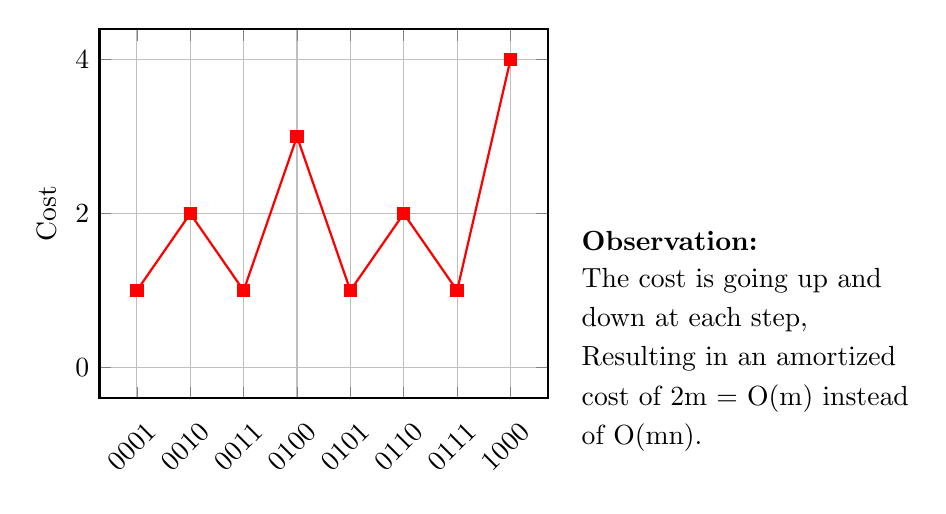
\begin{tikzpicture}
        \begin{axis}[
            width=0.6\textwidth, % Makes the plot narrower to leave space on the right
            xlabel={},
            ylabel={Cost},
            xtick={1,2,3,4,5,6,7,8},
            xticklabels={{0001}, {0010}, {0011}, {0100}, {0101}, {0110}, {0111}, {1000}}, 
            ymin=0, ymax=4,
            xtick distance=1, 
            grid=major,
            thick,
            enlargelimits=0.1, 
            x tick label style={rotate=45, anchor=north east, yshift=-4pt}, 
            scaled x ticks=false 
        ]
        \addplot[
            color=red,
            mark=square*,
            mark options={fill=red}
        ] coordinates {
            (1,1) (2,2) (3,1) (4,3) (5,1) (6,2) (7,1) (8,4)
        };
        \end{axis}

        % Add text on the right
        \node[anchor=west] at (6,2) {\textbf{Observation:}};
        \node[anchor=west] at (6,1.5) {The cost is going up and };
        \node[anchor=west] at (6,1) { down at each step,};
        \node[anchor=west] at (6,0.5) {Resulting in an amortized};
        \node[anchor=west] at (6,0) {cost of 2m = O(m) instead};
        \node[anchor=west] at (6,-0.5) {of O(mn).};
        
    \end{tikzpicture}
\end{frame}



\begin{frame}{Dijkstra’s Limitations}
    \begin{itemize}
        \item Can not handle negative weights.
    \end{itemize}

\end{frame}

\begin{frame}{Dijkstra’s Limitations}
    \begin{center}
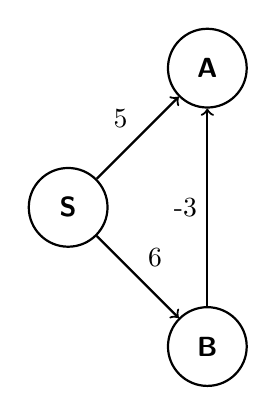
\begin{tikzpicture}[auto, node distance=2.5cm, thick, 
    main node/.style={circle, draw, fill=white!50, font=\sffamily\bfseries, minimum size=1cm}]

    % Define Nodes
    \node[main node] (S) {S};
    \node[main node] (A) [above right of=S] {A};
    \node[main node] (B) [below right of=S] {B};

    % Define Edges with Weights
    \path[->, thick]
        (S) edge node {5} (A)
        (S) edge node {6} (B)
        (B) edge node {-3} (A);
        
\end{tikzpicture}
\end{center}
\end{frame}

\begin{frame}{Dijkstra’s Limitations}
    \node{
        \only<1>{\textbf{Step 1: Start with S (Goal is A)}}
        \only<2>{\textbf{Step 2: Updating Neighbors of S}}
        \only<3>{\textbf{Step 3: Selecting A :Smallest Distance (Goal Reached!)}}
        \only<4>{\textbf{Incorrect Shortest Distance}}
        \only<5>{\textbf{The Real Shortest Distance}}
    };

    \begin{center}
        \begin{tikzpicture}[auto, node distance=2cm, thick, 
            main node/.style={circle, draw, fill=gray!10, font=\sffamily\bfseries, minimum size=1cm},
            eliminated node/.style={circle, draw, fill=gray!30, font=\sffamily\bfseries, minimum size=1cm},
            visited node/.style={circle, draw, fill=red!50, font=\sffamily\bfseries, minimum size=1cm},
            updated node/.style={circle, draw, fill=green!50, font=\sffamily\bfseries, minimum size=1cm},
            label node/.style={fill=yellow, font=\sffamily\small, inner sep=2pt},
            edge highlight/.style={draw=red, very thick},
            update edge/.style={draw=green, dashed, thick},
            >=stealth]

        % Nodes
        \node[main node] (S) {S};
        \node[main node, above right=1.5cm and 2cm of S] (A) {A};
        \node[main node, below right=1.5cm and 2cm of S] (B) {B};

        % Edges
        \path[->, thick] (S) edge node[label node] {5} (A);
        \path[->, thick] (S) edge node[label node] {6} (B);
        \path[->, thick] (B) edge node[label node] {-3} (A);

        % Step 1: Start at S
        \only<1>{\node[visited node] at (S) {S};
        \node[draw=green, thick] at ([xshift=-0.8cm]S) {0};
        \node[draw=green, thick] at ([xshift=-0.8cm]A) {$\infty$};
        \node[draw=green, thick] at ([yshift=-0.8cm]B) {$\infty$};
        }

        % Step 2: Update Neighbors of S
        \only<2>{
            \node[eliminated node] at (S) {S};
            \node[draw=green, thick] at ([xshift=-0.8cm]A) {5};
            \node[draw=green, thick] at ([yshift=-0.8cm]B) {6};
            \path[update edge] (S) -- (A);
            \path[update edge] (S) -- (B);
        }

        % Step 3: Select A :Smallest Distance (Goal Reached!)
        \only<3>{\node[visited node] at (A) {A};
        \node[eliminated node] at (S) {S};
        \node[draw=green, thick] at ([xshift=-0.8cm]A) {5};
        \node[draw=green, thick] at ([yshift=-0.8cm]B) {6};
        \path[edge highlight] (S) -- (A);
        }

        % Step 4: Select B (Smallest Distance)
        \only<4>{\node[visited node] at (A) {A};
        \node[eliminated node] at (S) {S};
        \node[draw=green, thick] at ([xshift=-0.8cm]A) {5};
        \node[draw=green, thick] at ([yshift=-0.8cm]B) {6};
        \path[edge highlight] (S) -- (A);
        
        }

        % Step 5: Failure to Update A Again
        \only<5>{
            \node[visited node] at (A) {A};
        \node[draw=green, thick] at ([xshift=-0.8cm]A) {3};
        \node[draw=green, thick] at ([yshift=-0.8cm]B) {6};
        \path[edge highlight] (S) -- (B);
        \path[edge highlight] (B) -- (A);
        \node[eliminated node] at (S) {S};
        \node[eliminated node] at (B) {B};
        }

        \end{tikzpicture}
    \end{center}
\end{frame}

\begin{frame}{Why Dijkstra’s Algorithm Failed?}
  
        \begin{itemize}
            \item Dijkstra assumes all edge weights are \textbf{non-negative}.
            \item \textbf{The negative weight edge} (B → A, cost = -3) breaks this assumption.
            \item Once a node is visited in Dijkstra’s algorithm, it is \textbf{never reprocessed}, leading to incorrect results.
            \item In this case, the shortest path S → B → A (cost=3) is \textbf{never found}, as Dijkstra \textbf{incorrectly finalizes} d(A)=5 \textbf{too early}.
        \end{itemize}
   
\end{frame}



\begin{frame}{Applications of Dijkstra’s Algorithm}
   
        \begin{itemize}
            \item \textbf{Network Routing:} Finding shortest paths in computer networks.
            \item \textbf{GPS \& Navigation:} Used in Google Maps to find the shortest routes.
            \item \textbf{Social Networks:} Finding the shortest connection path between users.
            \item \textbf{Airline Route Optimization:} Finding the cheapest travel routes.
        \end{itemize}
    
\end{frame}



\end{document}